\documentclass[11pt]{article}
\usepackage[margin=1in]{geometry}
\usepackage{amsmath,amssymb,bm}
\usepackage{booktabs}
\usepackage{array}
\usepackage{multirow}
\usepackage{graphicx}
\usepackage[hidelinks]{hyperref}
\usepackage{titlesec}

% structured headings (plain, no colour)
\titleformat{\section}{\large\bfseries}{\thesection.}{0.6em}{}
\titlespacing*{\section}{0pt}{1.5em}{0.5em}
\titleformat{\paragraph}[runin]{\normalfont\bfseries}{}{0em}{}

% Local section numbering: S1, S2, ...
\renewcommand{\thesection}{S\arabic{section}}
\renewcommand{\thetable}{S\arabic{table}}
\renewcommand{\thefigure}{S\arabic{figure}}

\title{\textbf{Supplementary Material}\\[2pt]
TARVI: Transcription-Factor Aided RNA Velocity Inference with\\
Supervised Latent Time and Velocity-Pseudotime Blending}
% \author{Chandula Adhikari \and Sandeep Dassanayake \and Damayanthi Herath\\
% \textit{Department of Computer Engineering, University of Peradeniya}}
% \date{}

\begin{document}
\maketitle

This supplement gives the full component ablation that the main paper summarises. We
first set out the background theory the analysis builds on---the closed-form kinetics
and the velocity-graph pseudotime that TARVI uses---at a level of detail condensed in
the main text, then present the ablation and the reproducibility and scope notes that
follow from it. Section and table numbering carry an \textbf{S} prefix and are local
to this document.

%==============================================================================
\section{Background Theory}
\label{sec:theory}
%==============================================================================

\paragraph{Closed-form four-state kinetics.} TARVI inherits VeloVI's two-branch
solution of the splicing ODEs, which the main text states only in words. With
transcription, splicing and degradation rates $\alpha,\beta,\gamma$ and a per-gene
switching time $t_s$, the induction branch starts from $u{=}s{=}0$ and evolves over
$t_{\text{ind}}=t_s\rho_{i,g}$ as
\begin{align}
u_{\text{ind}}(t) &= \tfrac{\alpha}{\beta}\big(1-e^{-\beta t}\big), &
s_{\text{ind}}(t) &= \tfrac{\alpha}{\gamma}\big(1-e^{-\gamma t}\big)
 + \tfrac{\alpha}{\gamma-\beta}\big(e^{-\gamma t}-e^{-\beta t}\big),
\label{eq:induction}
\end{align}
and the repression branch starts from the induction endpoint
$(u_0,s_0)=(u_{\text{ind}}(t_s),s_{\text{ind}}(t_s))$ and evolves over
$t_{\text{rep}}=(t_{\max}-t_s)\tau_{i,g}$ as
\begin{align}
u_{\text{rep}}(t) &= u_0\,e^{-\beta t}, &
s_{\text{rep}}(t) &= s_0\,e^{-\gamma t}
 - \tfrac{\beta u_0}{\gamma-\beta}\big(e^{-\gamma t}-e^{-\beta t}\big),
\label{eq:repression}
\end{align}
(a small $\varepsilon$ regularises $\gamma-\beta$), with the steady-state branches as
in the main paper. The RNA velocity is $v=\beta u-\gamma s$ evaluated on these
curves; in TARVI $\alpha$ is the cell-specific, TF-regulated rate $\alpha_i$, so
Eqs.~\eqref{eq:induction}--\eqref{eq:repression} are evaluated per cell. These curves
are what the Gene-R$^2_\text{spl}$ metric scores, which is why the TF rate enters the
kinetic-fit discussion below.

\paragraph{Velocity-graph pseudotime.} The blending step builds its global coordinate
not from expression distances but from the \emph{velocity} transition graph. For each
cell $i$ and neighbour $j$ in its $k$NN set $\mathcal{N}(i)$, a directed transition
probability comes from the cosine alignment of the velocity $\mathbf{v}_i$ with the
displacement $\mathbf{s}_j-\mathbf{s}_i$,
\begin{equation}
\pi_{ij} \;=\;
\frac{\exp\!\big(\cos(\mathbf{v}_i,\ \mathbf{s}_j-\mathbf{s}_i)/\sigma\big)}
{\sum_{k\in\mathcal{N}(i)}\exp\!\big(\cos(\mathbf{v}_i,\ \mathbf{s}_k-\mathbf{s}_i)/\sigma\big)},
\qquad \sigma>0 ,
\label{eq:transition}
\end{equation}
giving a row-stochastic matrix that points downhill along the field~\cite{bergen2020scvelo};
$t^{\text{VPT}}$ is then the diffusion pseudotime~\cite{haghverdi2016dpt} from a root
cell, rescaled to $[0,1]$. Because $\Pi=[\pi_{ij}]$ is built from the
\emph{already-trained} velocities, the blend is a post-hoc step that leaves the
velocity field unchanged---the property the ablation exploits.

%==============================================================================
\section{Component Ablation}
\label{sec:ablation}
%==============================================================================

We ablate each of the three components---the TF-regulated rate (TF), the
velocity--time consistency loss (VTC), and the velocity-pseudotime blend (VPT)---across
all five datasets (pancreas, bone marrow, forebrain, chromaffin, scEU-organoid).
Table~\ref{tab:ablation} reports cross-dataset means for the VeloVI baseline; VeloVI
with the blend on its \emph{own} velocity graph (VeloVI\,$+$\,VPT); the full model
with one component removed; and full TARVI. We write $\Delta_c\,m$ for the change in a
metric $m$ when component $c$ is removed from the full model, and
$\delta_{\text{VPT}}\,m$ for the change from adding the blend to the raw VeloVI graph.

\begin{table}[h]
\centering
\caption{Component ablation: cross-dataset mean performance over all five datasets.
VeloVI\,$+$\,VPT applies the blend ($\beta{=}0.7$) to the unmodified VeloVI velocity
graph. Best per column among configurations in bold. All metrics $\uparrow$.}
\label{tab:ablation}
\resizebox{\textwidth}{!}{%
\begin{tabular}{lrrrrrrrr}
\toprule
Config & ICCoH & CBDir & VelConf & PT-Spear & PT-DistCorr & PT-Cons & RootAcc & Gene-R$^2_\text{spl}$ \\
\midrule
VeloVI               & 0.787 & 0.931 & 0.920 & 0.331 & 0.341 & 0.905 & 0.723 & 0.442 \\
VeloVI\,$+$\,VPT     & 0.787 & 0.931 & 0.920 & 0.714 & 0.724 & \textbf{0.986} & 0.658 & 0.442 \\
TARVI\,$-$\,TF       & 0.693 & 0.911 & 0.902 & \textbf{0.759} & \textbf{0.783} & 0.984 & 0.653 & 0.461 \\
TARVI\,$-$\,VTC      & \textbf{0.792} & \textbf{0.934} & \textbf{0.928} & 0.700 & 0.705 & \textbf{0.986} & 0.556 & 0.474 \\
TARVI\,$-$\,VPT      & 0.776 & 0.933 & 0.927 & 0.320 & 0.316 & 0.891 & \textbf{0.728} & \textbf{0.479} \\
TARVI (full)         & 0.776 & 0.933 & 0.927 & 0.747 & 0.772 & \textbf{0.986} & 0.671 & \textbf{0.479} \\
\bottomrule
\end{tabular}}
\end{table}

The three components act on different axes. \textbf{The blend supplies the pseudotime
ordering:} $\Delta_{\text{VPT}}(\text{PT-Spear})=0.747-0.320=0.427$, with every
velocity-field metric (ICCoH, CBDir, VelConf, Gene-R$^2_\text{spl}$) unchanged between
full and $-$VPT---exactly as the post-hoc construction of Eq.~\eqref{eq:transition}
predicts. The effect is largely model-agnostic: on the raw VeloVI graph it already
gives $\delta_{\text{VPT}}(\text{PT-Spear})=0.714-0.331=0.383$, and the gap between
VeloVI\,$+$\,VPT and full TARVI ($+0.033$) is the part specific to TARVI's velocity
field. We therefore treat the blend as an orthogonal enhancement that recovers a
well-ordered pseudotime from any reasonable velocity graph.

\textbf{The TF rate sharpens the velocity field} rather than the temporal coordinate:
$\Delta_{\text{TF}}$ is positive on ICCoH ($+0.083$), VelConf ($+0.025$) and CBDir
($+0.022$) but slightly negative on PT-Spear. Its kinetic-fit gain on the curves of
Eqs.~\eqref{eq:induction}--\eqref{eq:repression} is real but modest
($\Delta_{\text{TF}}(\text{Gene-R}^2_\text{spl})=0.018$), by design: the basal rate is
warm-started from VeloVI and frozen so the TF term is an incremental correction,
VeloVI's four-state mixture already fits per-gene spliced dynamics well, and the L1
penalty keeps the weights sparse. The cell-specific rate thus behaves as a
biologically grounded regulariser that improves field consistency more than it
inflates $R^2$. \textbf{The VTC loss improves temporal ordering and root/terminal
identification:} $\Delta_{\text{VTC}}(\text{PT-Spear})=0.047$ and, most clearly,
$\Delta_{\text{VTC}}(\text{RootAcc})=0.115$, with a negligible effect on the field
metrics ($\le 0.016$).

Finally, the blend weight $\beta$ is robust. The two endpoints of the convex blend
appear directly in the table---$\beta{=}0$ (time-head only) is TARVI\,$-$\,VPT
(PT-Spear $0.320$) and $\beta{=}1$ (pure velocity-graph pseudotime) is
VeloVI\,$+$\,VPT ($0.714$)---and the global value $\beta{=}0.7$ used throughout
(full TARVI, $0.747$) exceeds both. The learned time and the velocity-graph
pseudotime are therefore complementary, and $\beta{=}0.7$ is a safe interior operating
point chosen once on the pooled cross-dataset mean rather than tuned per dataset.

%==============================================================================
\section{Qualitative Comparison on Chromaffin and Forebrain}
\label{sec:qual}
%==============================================================================

Complementing the pancreas case study in the main paper, Figs.~\ref{fig:chromaffin}
and~\ref{fig:forebrain} show, for every method, the projected velocity streamlines
(top row) and the inferred latent time (bottom row) on the chromaffin (t-SNE) and
forebrain (UMAP) datasets; each panel is titled with its method. On both datasets
TARVI produces coherent streamlines together with a smooth $0\!\to\!1$ latent-time
gradient, consistent with its temporal-metric lead (chromaffin PT-Spear $0.807$,
forebrain $0.887$, versus $0.147$ and $0.342$ for VeloVI). VeloVI recovers a similar
field (chromaffin/forebrain CBDir $0.911$/$0.938$) but an uncalibrated time; TFvelo's
streamlines are directionally inconsistent (chromaffin CBDir $0.005$); and scVelo
dynamical and Velocyto give intermediate results.

\begin{figure}[h]
\centering
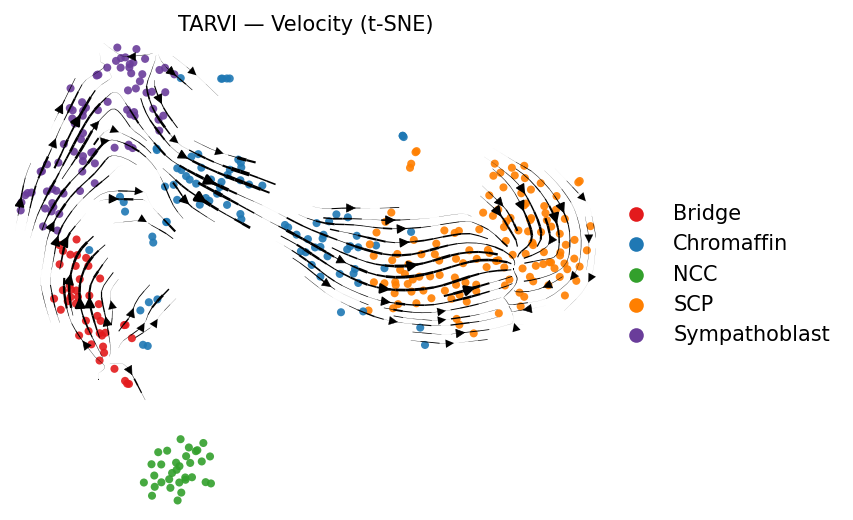
\includegraphics[width=0.19\linewidth]{figures/chromaffin/velocity_stream_TARVI.png}\hfill
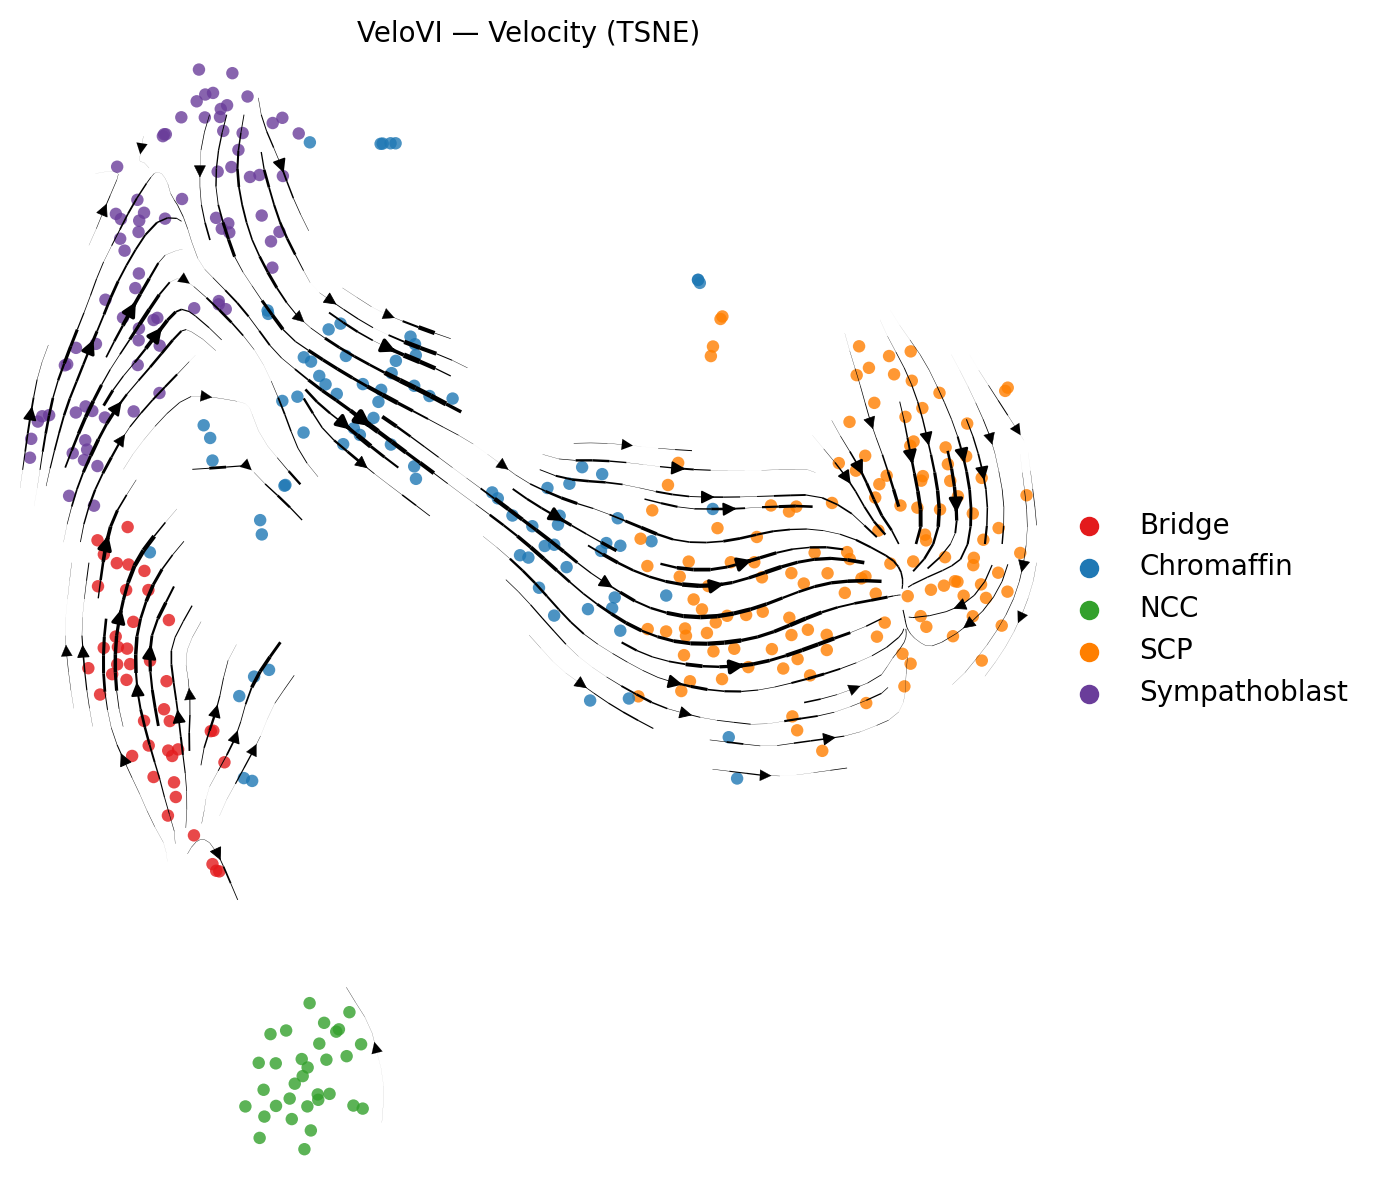
\includegraphics[width=0.19\linewidth]{figures/chromaffin/velocity_stream_VeloVI.png}\hfill
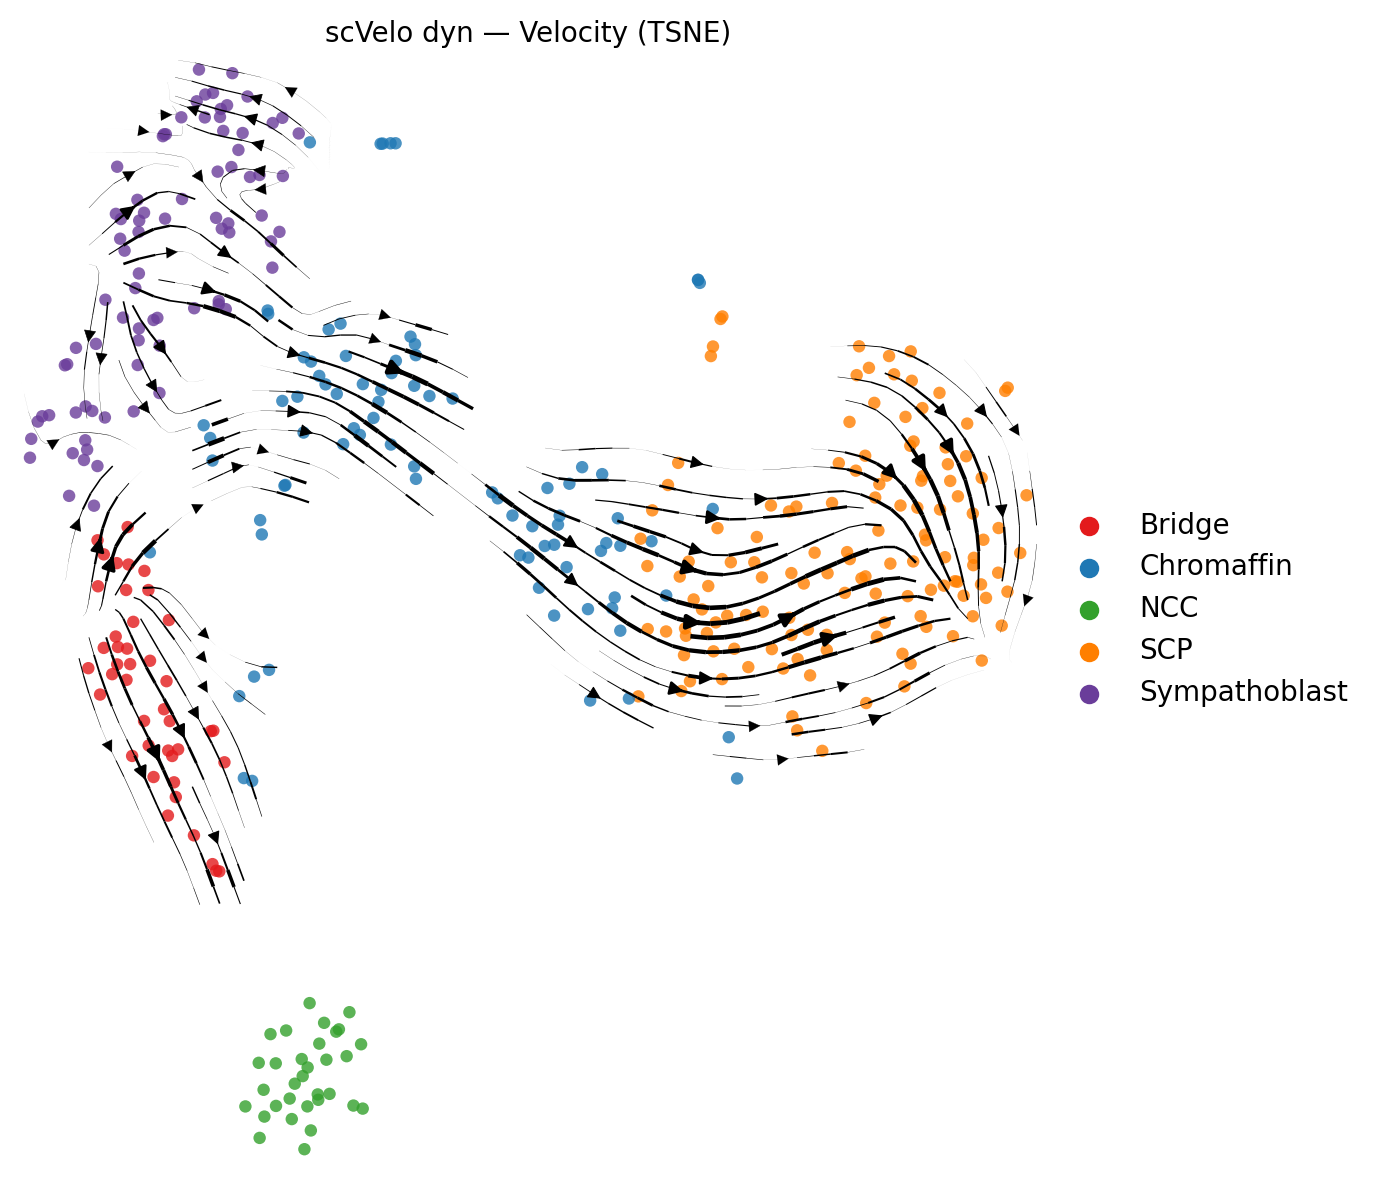
\includegraphics[width=0.19\linewidth]{figures/chromaffin/velocity_stream_scVelo_dyn.png}\hfill
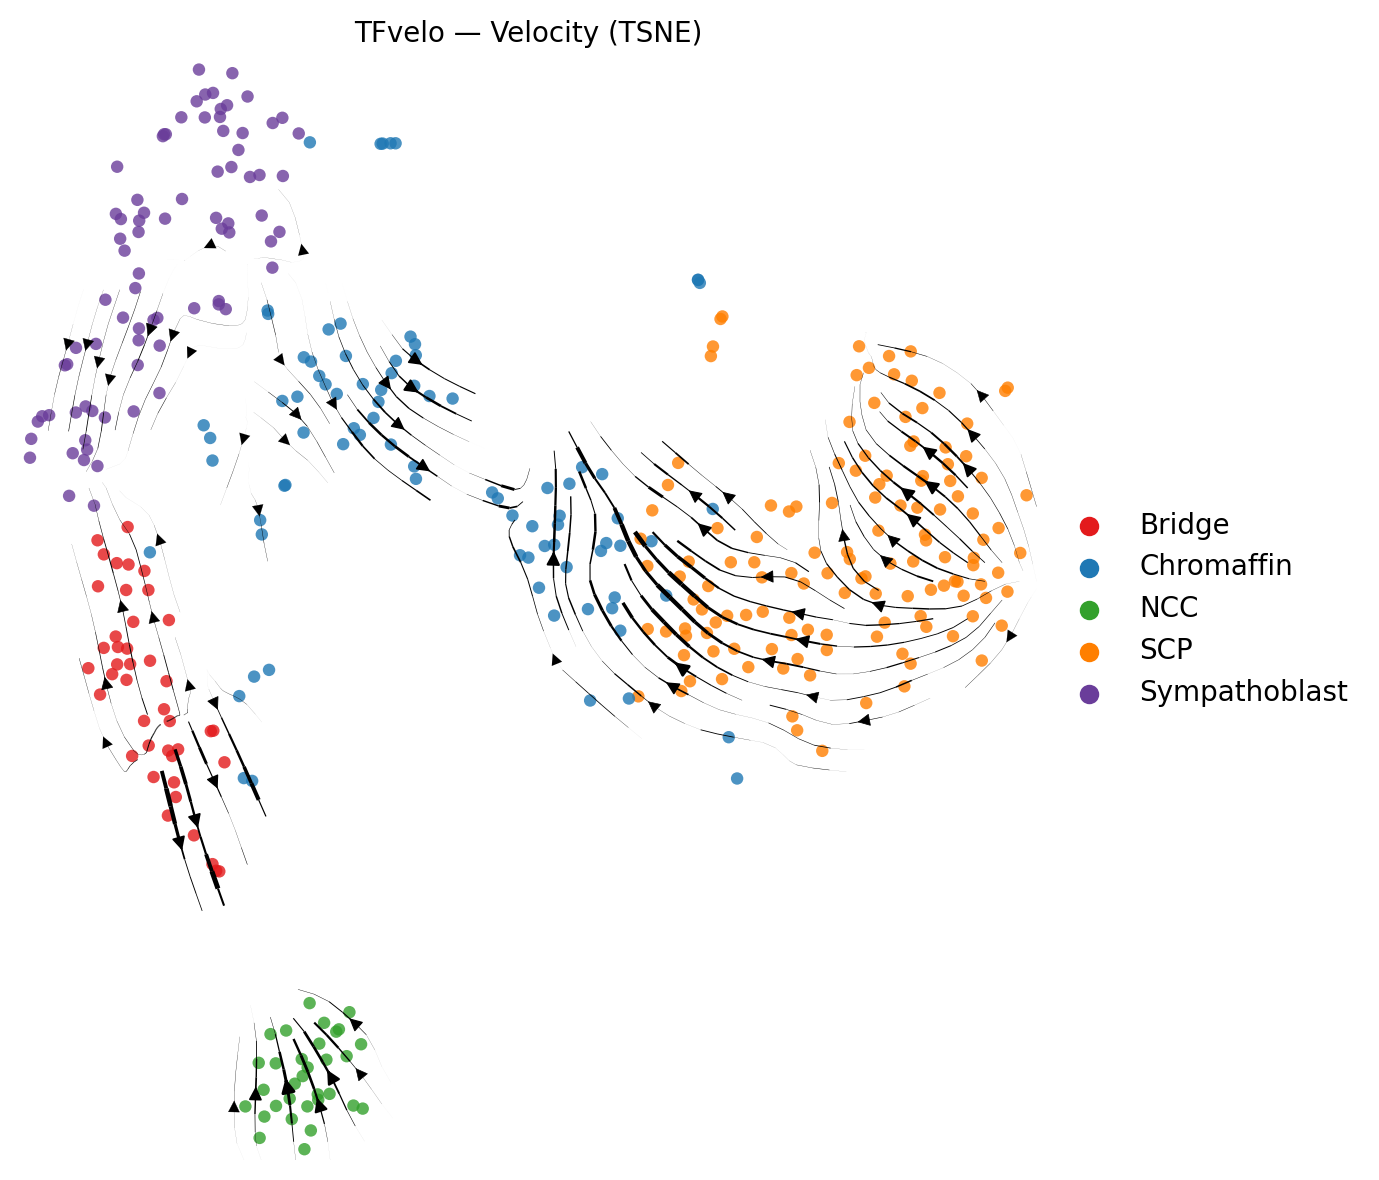
\includegraphics[width=0.19\linewidth]{figures/chromaffin/velocity_stream_TFvelo.png}\hfill

\includegraphics[width=0.19\linewidth]{figures/chromaffin/velocity_stream_velocyto.png}\\[3pt]
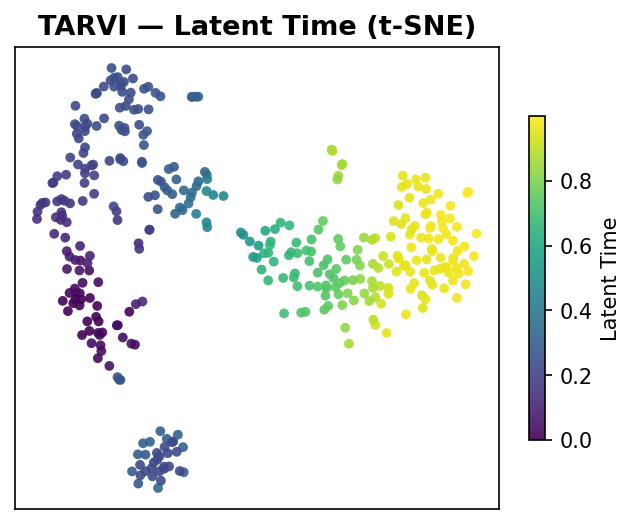
\includegraphics[width=0.19\linewidth]{figures/chromaffin/latent_time_TARVI.png}\hfill

\includegraphics[width=0.19\linewidth]{figures/chromaffin/latent_time_VeloVI.png}\hfill

\includegraphics[width=0.19\linewidth]{figures/chromaffin/latent_time_scVelo_dyn.png}\hfill
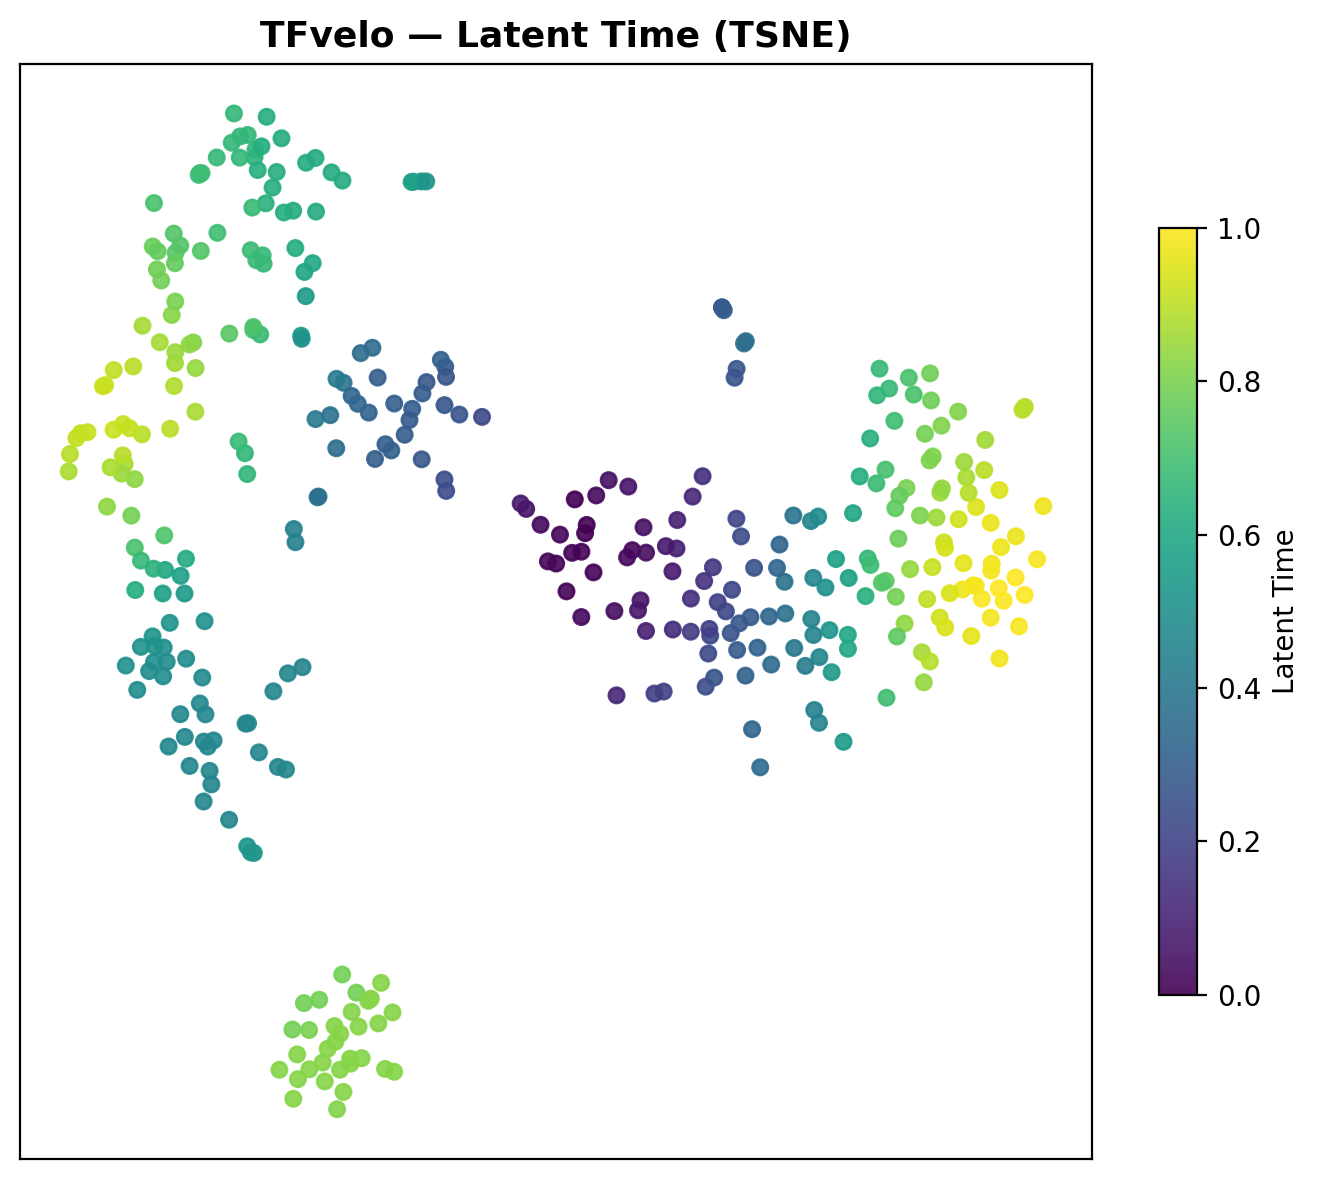
\includegraphics[width=0.19\linewidth]{figures/chromaffin/latent_time_TFvelo.png}\hfill
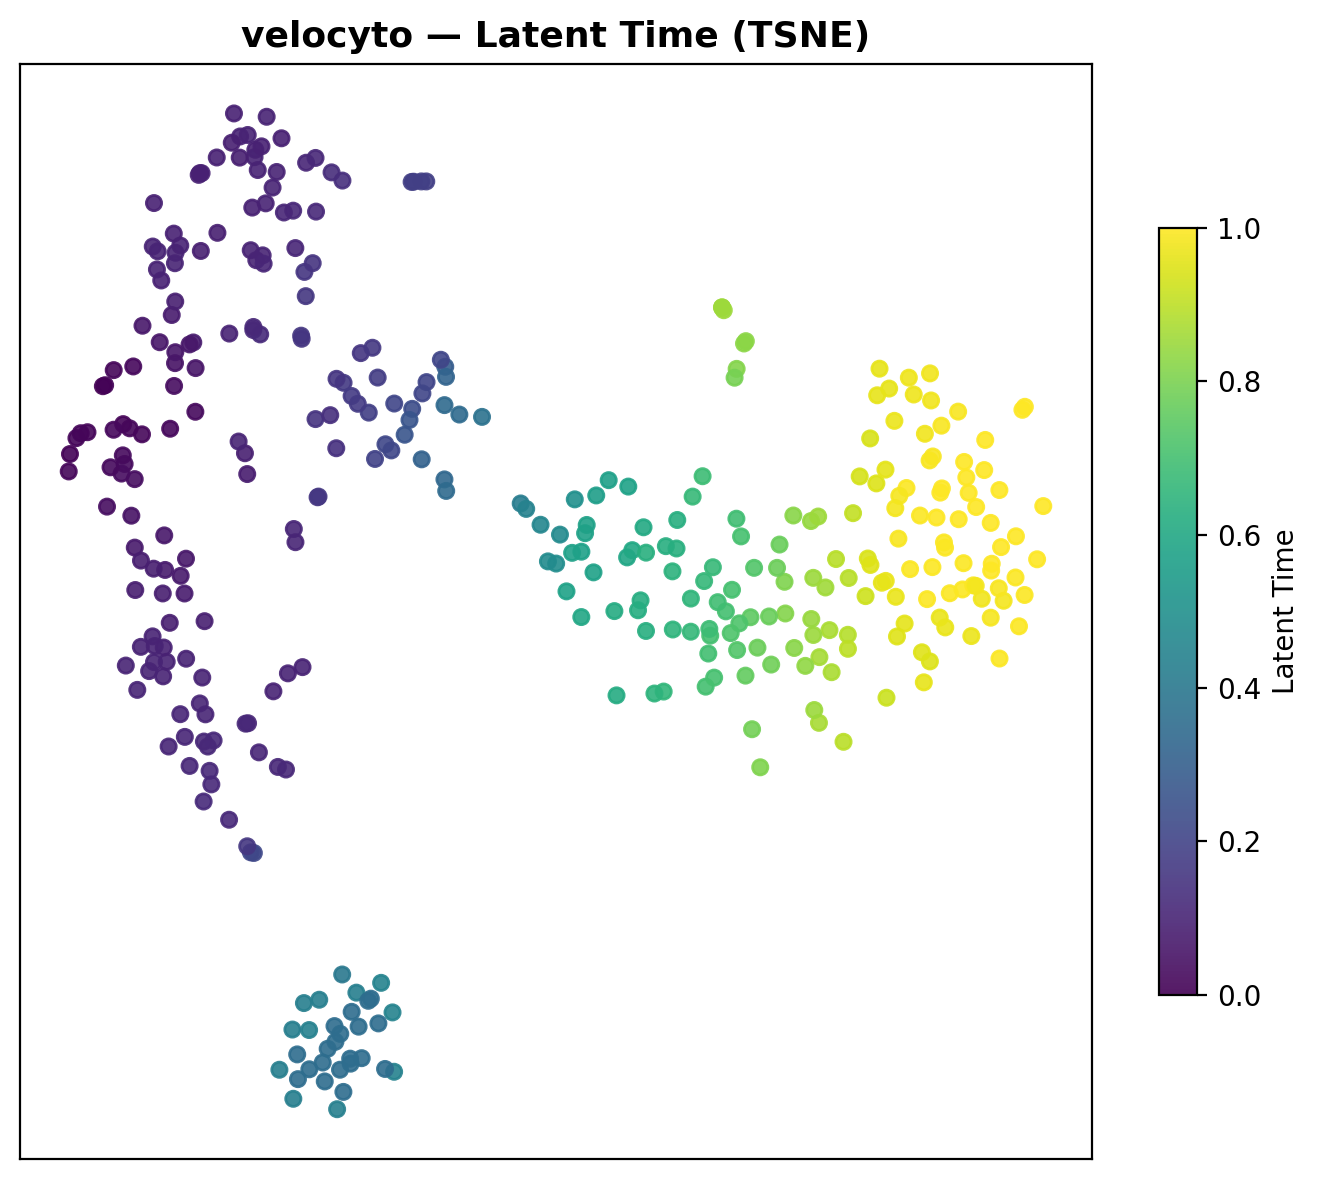
\includegraphics[width=0.19\linewidth]{figures/chromaffin/latent_time_velocyto.png}
\caption{Chromaffin (t-SNE): velocity streamlines (top) and inferred latent time
(bottom) for each method; panels are titled by method.}
\label{fig:chromaffin}
\end{figure}

\begin{figure}[h]
\centering

\includegraphics[width=0.19\linewidth]{figures/forebrain/velocity_stream_TARVI.png}\hfill

\includegraphics[width=0.19\linewidth]{figures/forebrain/velocity_stream_VeloVI.png}\hfill

\includegraphics[width=0.19\linewidth]{figures/forebrain/velocity_stream_scVelo_dyn.png}\hfill

\includegraphics[width=0.19\linewidth]{figures/forebrain/velocity_stream_TFvelo.png}\hfill

\includegraphics[width=0.19\linewidth]{figures/forebrain/velocity_stream_velocyto.png}\\[3pt]

\includegraphics[width=0.19\linewidth]{figures/forebrain/latent_time_TARVI.png}\hfill

\includegraphics[width=0.19\linewidth]{figures/forebrain/latent_time_VeloVI.png}\hfill

\includegraphics[width=0.19\linewidth]{figures/forebrain/latent_time_scVelo_dyn.png}\hfill

\includegraphics[width=0.19\linewidth]{figures/forebrain/latent_time_TFvelo.png}\hfill

\includegraphics[width=0.19\linewidth]{figures/forebrain/latent_time_velocyto.png}
\caption{Forebrain (UMAP): velocity streamlines (top) and inferred latent time
(bottom) for each method; panels are titled by method.}
\label{fig:forebrain}
\end{figure}

%==============================================================================
\section{Reproducibility, Statistical Reading, and Scope}
\label{sec:scope}
%==============================================================================

All results use a fixed random seed and a deterministic preprocessing pipeline, and
we report single-run point estimates. The values in Table~\ref{tab:ablation} come
from a dedicated ablation run and differ from the main-text headline numbers by
$\le 0.01$ on the aggregate means; comparisons within the table are internally
consistent. This $\le 0.01$ drift is the right scale for reading small differences:
gaps on that order---such as TARVI versus VeloVI on the directional metrics (CBDir,
VelConf)---should be read as comparable rather than as wins, whereas the pseudotime
contributions above ($\Delta_{\text{VPT}}\,\text{PT-Spear}=0.427$) are an order of
magnitude larger.

A few limitations bound the scope of these conclusions. We did not run a multi-seed
study, so we report no confidence intervals or paired significance tests; a
multi-seed analysis with paired tests across datasets is the natural next
step~\cite{liu2026benchmark}. The TF prior is rebuilt per dataset by intersecting the
ENCODE/ChEA databases with each gene panel; because such databases are incomplete and
tissue-context dependent, genes with no reliable TF edges fall back (through the
frozen basal rate and the L1 penalty) to VeloVI-like behaviour, so for lineages or
organisms outside the ENCODE/ChEA scope we expect TARVI to approach the no-TF regime
rather than to fail, and a systematic study of mask completeness is left to future
work. Finally, VeloTrace~\cite{cheng2026velotrace}, a concurrent method targeting the
same velocity--trajectory gap, has no public code release that would allow a faithful
re-implementation under our preprocessing and metric protocol, so we could not include
it among the baseline comparisons.

%==============================================================================
\begin{thebibliography}{9}
\bibitem{bergen2020scvelo} V. Bergen \emph{et al.}, ``Generalizing RNA velocity to
transient cell states through dynamical modeling,'' \emph{Nature Biotechnology},
vol.~38, pp.~1408--1414, 2020.
\bibitem{haghverdi2016dpt} L. Haghverdi \emph{et al.}, ``Diffusion pseudotime
robustly reconstructs lineage branching,'' \emph{Nature Methods}, vol.~13,
pp.~845--848, 2016.
\bibitem{liu2026benchmark} J. Liu \emph{et al.}, ``Comprehensive benchmarking of RNA
velocity methods across single-cell datasets,'' 2026.
\bibitem{cheng2026velotrace} H. Cheng \emph{et al.}, ``VeloTrace Reconciles
Divergent Velocity and Trajectory in Single-cell Transcriptomics with Deep Neural
ODE,'' \emph{bioRxiv}, 2026.
\end{thebibliography}

\end{document}
